\section{Модификация проекта «Изображение проекции полиэдра»}

\subsection*{Точная постановка задачи}
Модифицируйте эталонный проект таким образом, 
чтобы определялась и печаталась следующая характеристика полиэдра: 
сумма длин проекций полностью невидимых рёбер, центр которых находится 
строго внутри сферы $x^2+y^2+z^2=4$.

\subsection*{Решение данной задачи и модификация кода}
Для решения данной задачи модифицируем код файла $\texttt{shadow/polyedr.rb}$.
Проверка ребра на невидимость, а также проверка центра ребра на попадание в 
сферу и вычисление периметра суммы длин проекций выполняется в методе $\texttt{draw}$ класса $\texttt{Polyedr}$:


\begin{small}
\begin{verbatim}
class Polyedr 
  ...

  def draw
    ...
    p=0.0
      edges.each do |e|
        facets.each{|f| e.shadow(f)}
          e.gaps.each{|s| TkDrawer.draw_line(e.r3(s.beg), e.r3(s.fin))}
            if e.invisible?
              if e.func?(c)
                p+=e.perimeter(c)
              end
            end
      end
  return p
  end  
end
\end{verbatim}
\end{small}

Чтобы проверить, является ли ребро невидимым, нужно проверить является ли массив $\texttt{@gaps}$ пустым. Для этого 
добавим в файл $\texttt{shadow/polyedr.rb}$ метод $\texttt{invisible?}$ в классе $\texttt{Edge}$:
\begin{small}
\begin{verbatim}
class Edge 
  ...
  def invisible?
    @gaps.size==0 ? true : false
  end
  ...
end
\end{verbatim}
\end{small}
В файле $\texttt{common/polyedr.rb}$ дополним метод $\texttt{initialize(file)}$ в классе 
$\texttt{Polyedr}$ заведем константу с коэффициентом гомотетии:


\begin{small}
\begin{verbatim}
class Polyedr 
  ...
  def initialize(file)
    ...
    @c=c
    ...
  end
end
\end{verbatim}
\end{small}
Чтобы проверить находится ли центр полностью невидемых рёбер строго внутри сферы $x^2+y^2+z^2=4$ с учетом 
коэффициента гомотетии. Используем следующую формулу для проверки центра ребра:
$$x^2+y^2+z^2<4\,.$$
Надо добавить в файле $\texttt{shadow/polyedr.rb}$ 
метод $\texttt{func?(c)}$ в класс $\texttt{Edge}$:
\begin{small}
\begin{verbatim}
class Edge 
  ...
  def func?(c)
    point=r3(0.5)
    point.x**2+point.y**2+point.z**2 < 4*c**2
  end
  ...
end
\end{verbatim}
\end{small}


После чего нам необходимо посчитать суммы длин проекций. Суммы длин проекций с учетом коэффициента гомотетии
будем искать с помощью формулы:
$$\frac{\sqrt{(x_2-x_1)^2+(y_2-y_1)^2}}{\mathrm{c}} \,. $$



Добавим в файле $\texttt{shadow/polyedr.rb}$ метод $\texttt{perimetr(c)}$ в класс $\texttt{Edge}$, позволяющий вычислить длину проеции.

\begin{small}
\begin{verbatim}
class Polyedr 
  ...
  def perimeter(c)
    vx=@fin.x-@beg.x
    vy=@fin.y-@beg.y
    (Math.sqrt(vx**2+vy**2))/c
  end	
  ...
end
\end{verbatim}
\end{small}

Заключительная модификация в файле $\texttt{shadow/run\_polyedr.rb}$ $-$ вывод результата на экран:

\begin{small}
\begin{verbatim}
#!/usr/bin/env ruby
require_relative './polyedr'
require_relative '../common/tk_drawer'
TkDrawer.create
%w(ccc box cube king).each do |name|
  puts '============================================================='
  puts "Начало работы с полиэдром '#{name}'"
  start_time = Time.now
  a=Polyedr.new("../data/#{name}.geom")
  puts "Сумма длин проекций #{a.draw}"
  puts "Изображение полиэдра '#{name}' заняло #{Time.now - start_time} сек."
  print 'Hit "Return" to continue -> '
  gets
end
\end{verbatim}
\end{small}

Модификация эталонного проекта «Изображение проекции полиэдра» завершена. Пример работы программы 
с модифицированным файлом $\texttt{cube1.geom}$ можно увидеть на (рис.4) и его содержание представленно ниже.
\begin{figure}[ht!]
\begin{center}
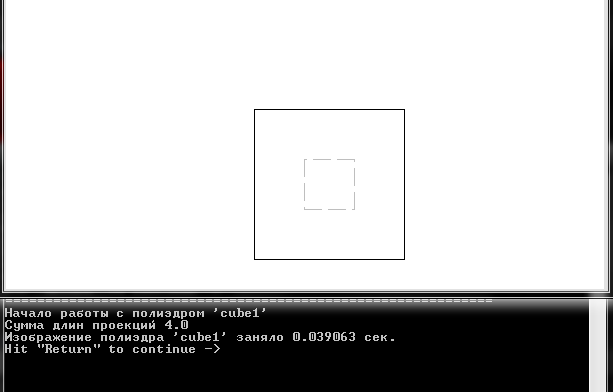
\includegraphics[width=0.8\hsize]{images/cube1}
\end{center}
\caption{Работа программы «Изображение проекции полиэдра»}\label{fig:polyedr}
\end{figure}
\newpage\begin{small}
\begin{verbatim}
50.0  0.0  0.0  0.0
 8  2  8
 0.0  0.0  0.0	
 1.0  0.0  0.0
 1.0  1.0  0.0	
 0.0  1.0  0.0	
-1.0 -1.0  1.0	
 2.0 -1.0  1.0	
 2.0  2.0  1.0	
-1.0  2.0  1.0	
4  1  2  3  4      
4  5  6  7  8
\end{verbatim}
\end{small}



